%
\section{Module-Based Domain Behavior Language}\label{sect:agl} %
The unified model is linked to an activity graph, which models the generic graph structure that is common to all activities. This activity graph incorporates module action to specialize the behavior of its nodes.
In the terminology of the DDD's layer architecture~\cite{evans_domain-driven_2004}, the activity graph is positioned at the application layer, because it coordinates the behaviors of the modules owning the domain classes in the unified model in order to perform the overall activity's behavior.

From the language engineering's perspective, we argue that the same benefits that are gained in unified domain modeling with \dcsl~can be attained for activity graphs if we develop a horizontal aDSL for them. We call this aDSL \abbrv{activity graph language}{\agl}.
The language is used to create activity graphs by \textit{configuring} them directly on the domain model using annotations. We call a model that conforms to \agl~an \abbrv{activity graph configuration}{AGC}.

Adapting the meta-modeling approach for DSLs~\cite{kleppe_software_2008}, we specify \agl~in terms of an \textit{abstract syntax meta-model} (ASM) and an annotation-based textual \textit{concrete syntax model (CSM)}. We also briefly discuss the semantics of \agl, relative to the activity graph and module action.
%
%More specifically, we construct the ASM in three steps. In the first step, we construct a conceptual model (CM) of the domain as a UML/OCL class diagram. This model helps understand the overall structure, without being constrained by the target OOPL's meta-model. The next two steps gradually transform CM into the ASM. In the second step, we transform CM into an equivalent, annotation-friendly form, called CM$_T$. In order to reduce the size of the eventual ASM, we try, in this step, to produce a compact CM$_T$. In the third step, we then transform CM$_T$ into the actual ASM, which takes an annotation-based form specified by the OOPL's meta-model. In this form, the configuration-related meta-concepts are represented by annotations. Further, we use Class as the basis to structure the annotations. 
%%%%%%%%%%%%%%%%%%%%%%%%%%%%%%%%%%%%%%%%%%%%%%%%%%%
\subsection{Abstract Syntax} \label{sect:agl-abstractSyntax}
%%%%%%%%%%%%%%%%%%%%%%%%%%%%%%%%%%%%%%%%%%%%%%%%%%%

We describe the \agl's domain requirements in terms of the following inclusion (I), exclusion (X) and restriction (R) clauses that are applied to the UML activity graph requirements stated in Chapters 15 and 16 of the UML specification~\cite{omg_unified_2015}:

%TODO: + Domain 
% + Exclude guards on Edge (is this already realized in the code? or future work?)
% + I1: include Module Action as described in previous section
% + R2: Executable node is a module action 
\begin{itemize}%[leftmargin=15pt]
	\item[I1.] module action (described in Section~\ref{sect:actSemantics}) as a special form of action.
	\item[R1.] executable node performs a sequence of module actions.
	\item[R2.] value specification (\S{15.2.3.3}, pg.~374) is only applied to decision node.
	\item[X1.] using variable with activity (\S{15.2.3.5}, pg.~417).
	\item[X2.] variable action (\S{16.9}, pg.~467).
  \item[X3.] activity edge (\S{15.2.3.3}, pg.~373) is without guards.
\end{itemize}

I1 and R1 are needed to incorporate activity graph into MOSA. R2 is a safe restriction because, according to the specification, value specification is mainly used for specifying conditions on decision node. X1 and X2 concern the use of variables. According to the UML specification, variable is alternative to using object flow. The exclusion of edge guards in X3 is not a limitation of our approach. It is a deliberate omission at this stage when we want to focus on supporting the core structure of the activity graph. We plan to remove X3 in future work.
%
%\subsection{Conceptual Model (CM)} \label{sect:agl-conceptual-model}
% TODO: + CM
% + rewrite to follow this structure: Conceptual model -> Abstract Syntax (CMt, The Annotation-based ASM)
% + Fig.: reposition the stereotype <<interface>>
% + Appstate: -> State
%   + an enum that captures all the states and concurrent states
% + ModuleAct:
%   + add attributes: preStates and output (Note: values of both attributes are pre-defined and need not be set by the user)
%   + fieldValSet: add ModuleAct.fieldVals (default to be empty - either no input or input vals come from internal of the system (e.g. another action) and not from the user))
% + Node:
%   + refCls: Class<DomainClass>
%   ? serviceCls: 
%     ? check that ModuleService and its ModuleActs are implemented correctly in jDomainApp
%
\begin{figure*}[ht]
	\begin{center}
		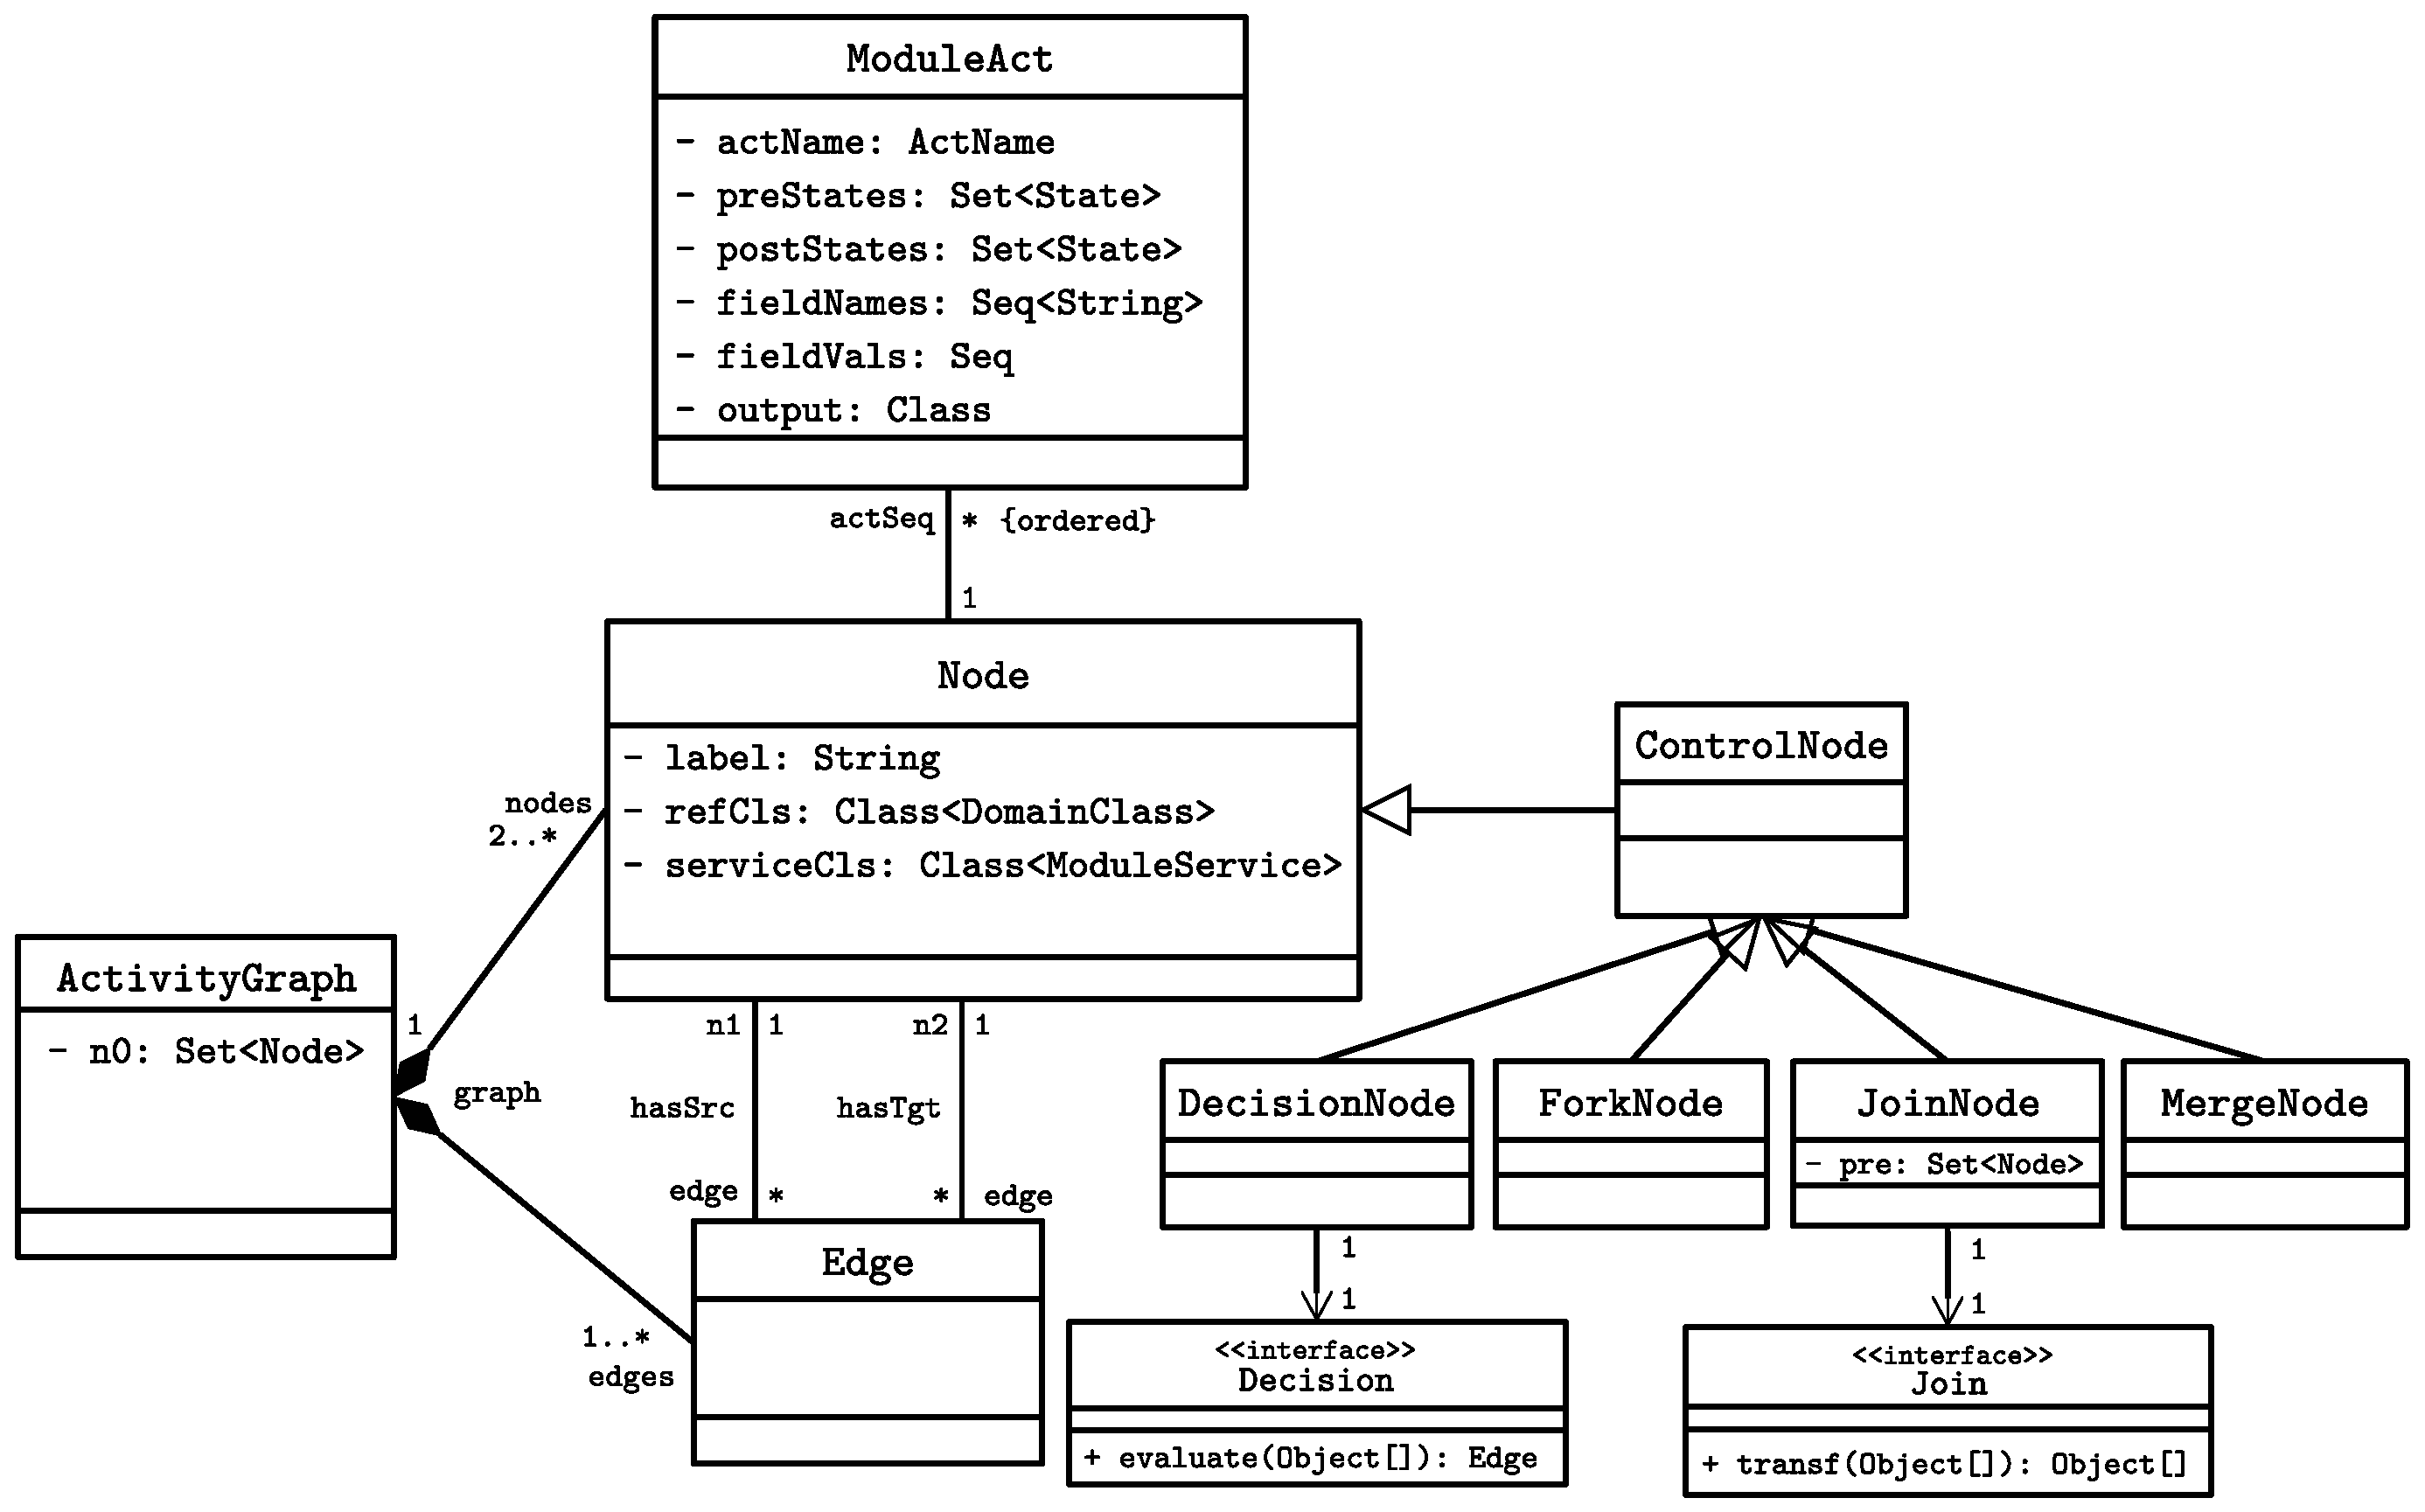
\includegraphics[scale=0.33]{agl-cm}
	\end{center}
	\caption{The metamodel ASM for the abstract syntax of \agl.} %
	\label{fig:agl-abstractSyntax}
\end{figure*}

% TODO: + CM rules
% + add rules for ModuleAct.preStates, fieldNames, fieldVals
% + add rules on refCls for JoinNode, DecisionNode and other nodes
% + Node:
%   + serviceCls: add OCL constraint on ModuleService.methods, whose names match those of the associated ModuleActs

We define the abstract syntax of \agl~with a metamodel as shown in Figure~\ref{fig:agl-abstractSyntax}. The well-formedness OCL rules of this model are presented in~\ref{apex:agl-rules}. To unify the notation with the unified model, in the text we will express the concepts of this model using the equivalent \dcsl's terms (see Section~\ref{sect:bg-dcsl}). This is possible because the model only contains elements (class, attribute, one-one and one-many associations and generalization) that are expressible by \dcsl.
%
The following paragraphs describe the main meta-concepts of the ASM. Note that we use an enumeration called \clazz{ActName} and an enumeration called \clazz{State} to represent the action names and the union of pre-states and post-states (\resp). \clazz{State}, in particular, represents both normal states and concurrent states (see Section~\ref{sect:arch-atomic-action}).
%
\begin{description}
%\subsubsection*{\clazz{ModuleAct}}\label{sect:agl-cm-moduleact}
\item[\clazz{ModuleAct}.] This represents SAA-typed module actions as defined in Definition~\ref{def:saa}. Field \attribn{actName} realizes the action name. The three fields \attribn{preStates}, \attribn{postStates}, and \attribn{output} realize three similarly-named attributes of the action.
%
The two fields \attrib{ModuleAct}{fieldNames} and  \attribn{fieldVals}  together realize the attribute \membern{fieldValSet} of the action, as follows: each pair $ (f,v) $ in \membern{fieldValSet} is constructed by taking $f$ from \attribn{fieldNames} and $v$ from the corresponding element of \attribn{fieldVals}.
%
%\subsubsection*{\clazz{ActivityGraph}}\label{sect:agl-cm-activity-graph}
\item[\clazz{ActivityGraph}.] This represents activity graphs and has three fields: \attribn{nodes}, \attribn{edges}, and \attribn{n0}. The first two fields are associative fields that realize the associations to \clazz{Node} and \clazz{Edge} (\resp). Field \attribn{n0} realizes a sub-set of nodes that are the start nodes of the graph. The starting nodes are the ones that are invoked first when the graph is executed.
%
%\subsubsection*{\clazz{Node}} \label{sect:agl-cm-ctrl-node}
\item[\clazz{Node}.] This represents activity nodes and has four fields. Field \attribn{label} realizes the node label. 
%Field \attribn{out} is derived from the association \clzassoc{hasSrc}{Edge}{Node}, which records the outgoing edges from a \clazz{Node}. 
The next two fields specify the \textbf{referenced (abbrv. \textit{ref}) software module}, i.e., the module that is referenced by this node. Specifically, field \attribn{refCls} (typed \clazztpl{Class}{\clazz{DomainClass}}) specifies the domain class of the \textit{ref} module. We call this class the \textit{ref} domain class. Here, we assume \clazztpl{Class}{\clazz{DomainClass}} represents the Domain Class concept of \dcsl~(see Section~\ref{sect:bg-dcsl}).

Field \attribn{serviceCls} (typed \clazztpl{Class}{\clazz{ModuleService}}) specifies the actual \clazz{ModuleService} class of the \textit{ref} software module. 
A default module service class for action nodes that we developed as part of the \jdomainapp~framework~\cite{le_jdomainapp_2017} is a class named \clazz{DataController}.
It is through a module service object of \attribn{serviceCls} that the current \clazz{Node} is able to perform the \clazz{ModuleAct}s specified by the field \attribn{actSeq}. This field is an associative field that realizes the the association from \clazz{Node} to \clazz{ModuleAct}.
%
%\subsubsection*{\clazz{ControlNode}} \label{sect:agl-control-node}
\item[\clazz{ControlNode}.] This is an abstract sub-type of \clazz{Node} that represents the control nodes of the activity graph. This class is used to specify behavior of control nodes and to capture the state of its execution. We specialize class \clazz{ControlNode} into the four sub-types: \clazz{DecisionNode}, \clazz{ForkNode}, \clazz{JoinNode}, and \clazz{MergeNode}. 
In particular, class \clazz{DecisionNode} references an interface named \clazz{Decision}, which provides a method (named \membern{evaluate}) for evaluating the decision logic. Similarly, class \clazz{JoinNode} references interface \clazz{Join}, which has a method (named \membern{transf}) for transforming the input tokens into output ones (if needed).
Further, class \clazz{JoinNode} has a field named \attribn{pre}, which is a derived field that realizes the source \clazz{Node}s of the activity edges connecting to a \clazz{JoinNode}.

Actual implementations of the interfaces \clazz{Decision} and \clazz{Join} are provided in the corresponding decision and join classes (\resp) in the unified model.
%
%\subsubsection*{\clazz{Edge}} \label{sect:agl-cm-edge}
\item[\clazz{Edge}.] This represents activity edges. It has two associative fields \attribn{n1} and \attribn{n2}, which realize the two associations to \clazz{Node}. Field \attribn{n1} captures the source node, while field \attribn{n2} captures the target one. Intuitively, there is a correspondence between an \clazz{Edge} and an association between the two domain classes that are referenced by the source and target nodes of the edge.
\end{description}

\begin{figure}[ht]
	\centering
	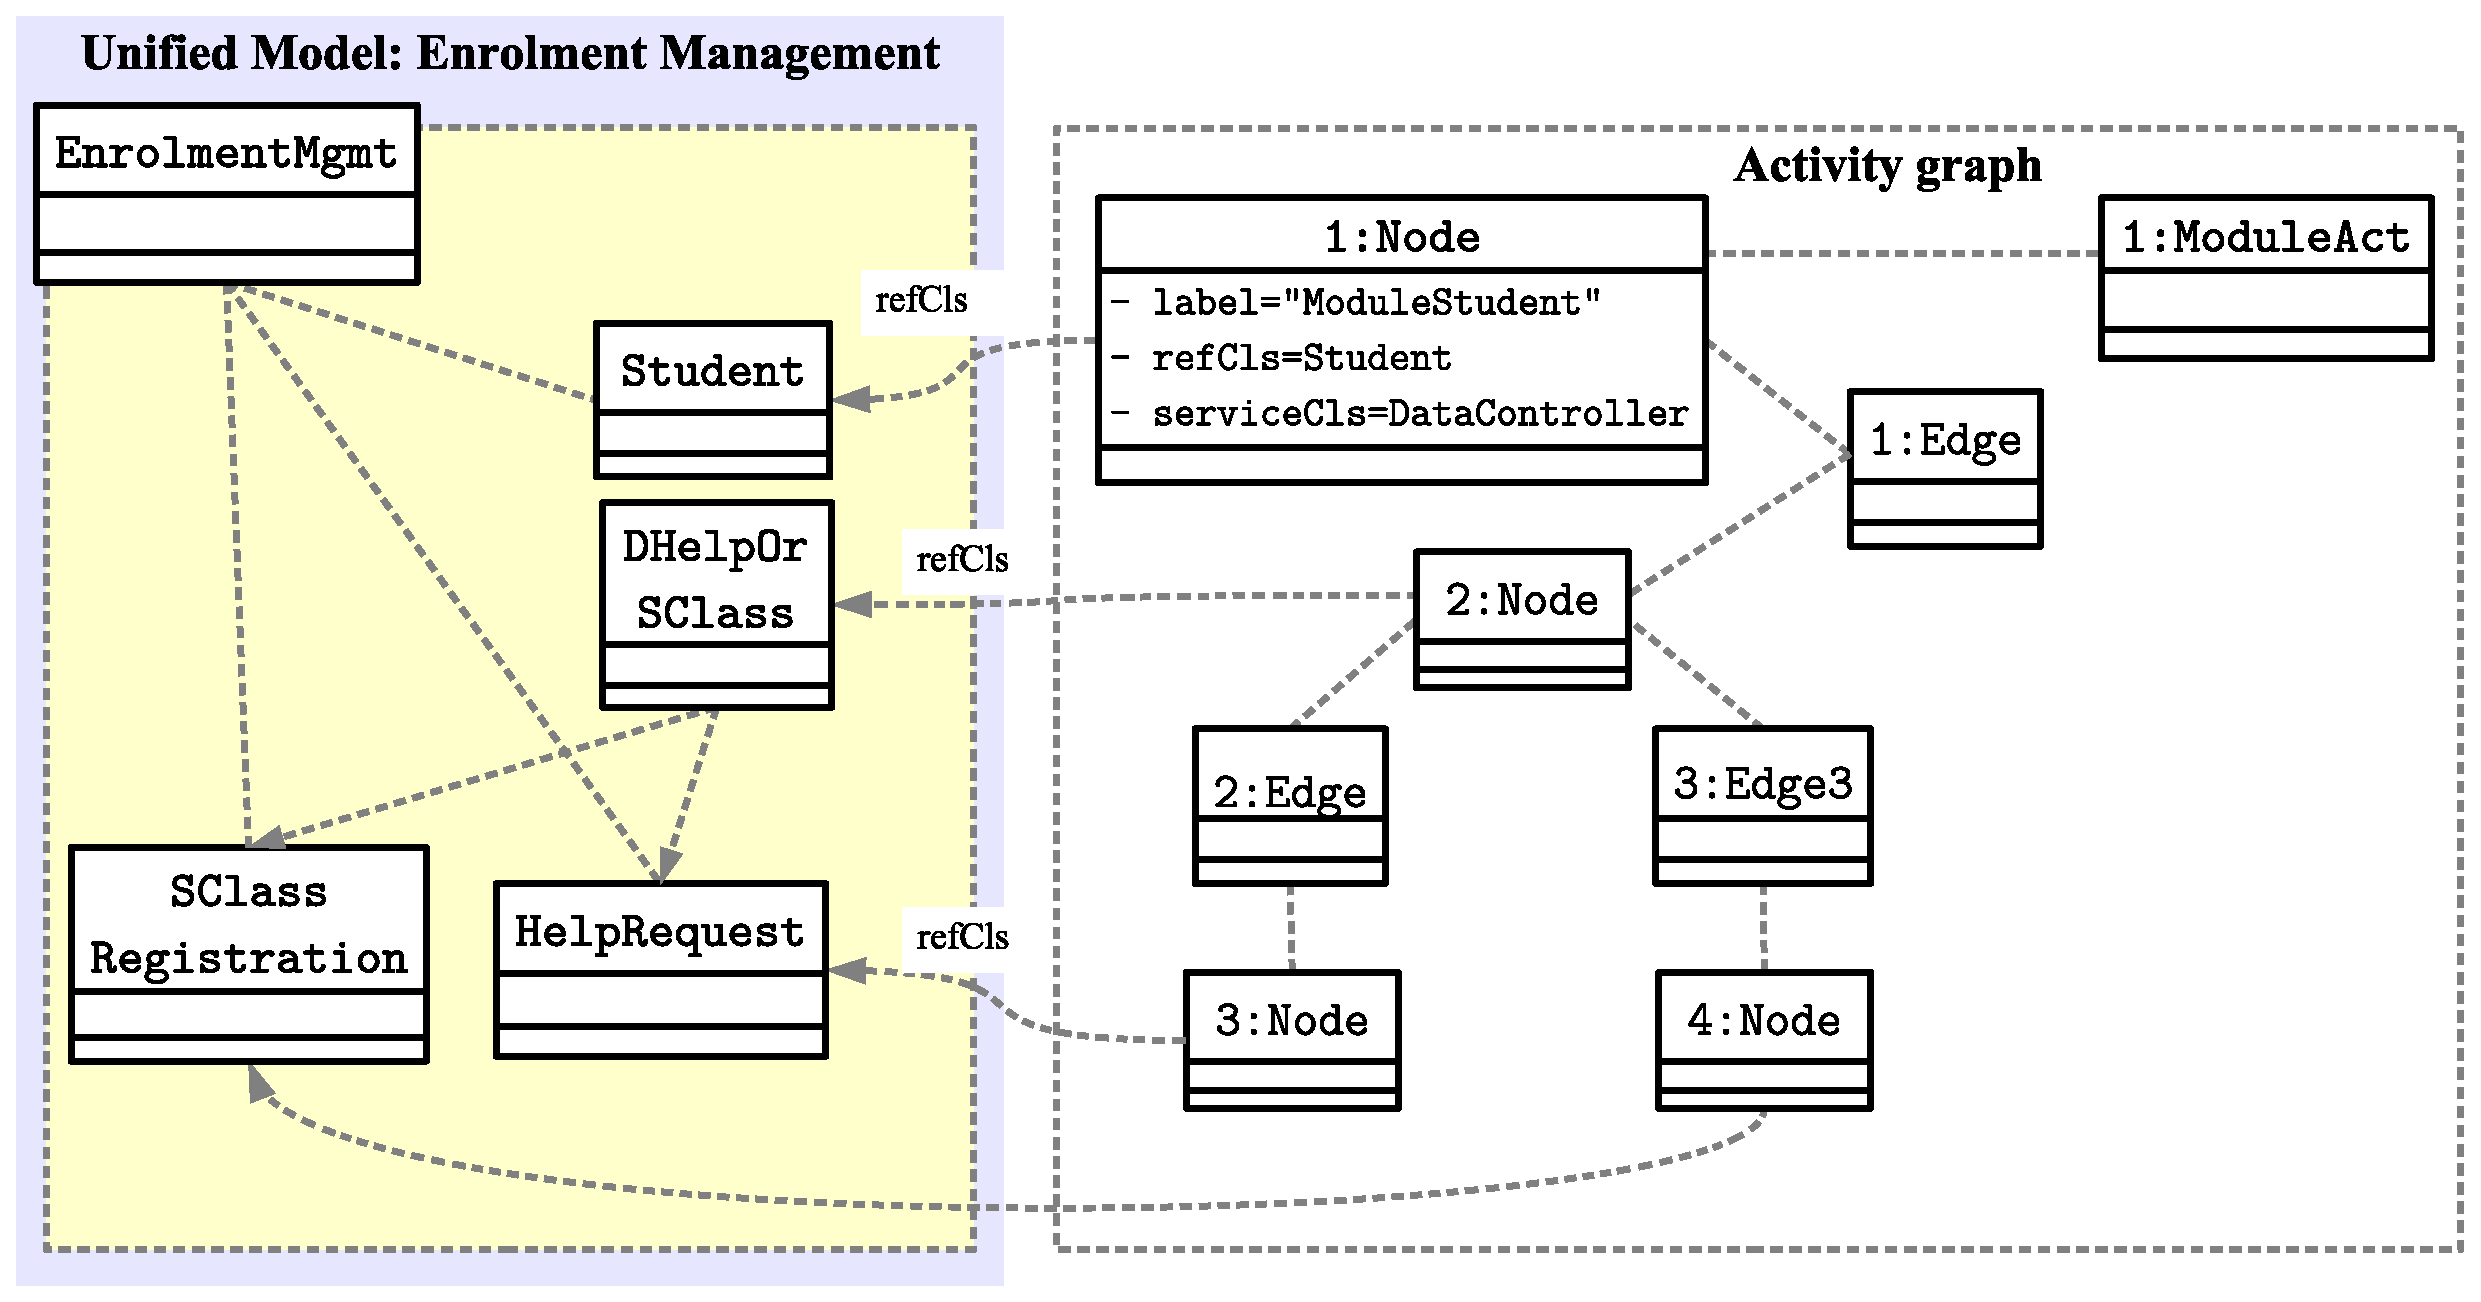
\includegraphics[scale=0.3]{activity-graph-example}
	\caption{(LHS) A repeat of the unified model shown in Figure~\ref{fig:unified-model-example}; (RHS) The activity graph of this model.} %
	\label{fig:activity-graph-example}
\end{figure}
%
% TODO: + tab:activity-graph-example
% + add a separate table for ModuleAct objects and reference them in the actSeq column
\begin{table*}[ht]
	\setlength\tabcolsep{5pt}
	\begin{center} \footnotesize
		\caption{(A: Top) \clazz{Node} objects, (B: Bottom-left) \clazz{Edge} objects of the activity graph in Figure~\ref{fig:activity-graph-example} and (C: Bottom-right)  
    \clazz{ModuleAct} objects that are referenced by the \clazz{Node}s}\label{tab:activity-graph-example}
    %
		\begin{tabular}{|>{\centering\arraybackslash}m{0.7cm}|>{\centering\arraybackslash}m{3.5cm}|>{\centering\arraybackslash}m{3cm}|>{\centering\arraybackslash}m{2.5cm}|>{\centering\arraybackslash}m{5cm}|}
			%content
			\hline
			\rowcolor{lightgray}
			\textbf{Node-Id} & \textbf{\attribn{label}} & \textbf{\attribn{refCls}} & \textbf{\attribn{serviceCls}} & \textbf{\attribn{actSeq}} \\\hline
			1 & \strq{MStudent} & \clazz{Student} & \clazz{DataController} & [\objid{1}{ModuleAct}]\\\hline 
			2 & \strq{MDHelpOrSClass} & \clazz{DHelpOrSClass} & \code{null} & \code{null}\\\hline 
			3 & \strq{MHelpRequest} & \clazz{HelpRequest} & \clazz{DataController} & [\objid{2}{ModuleAct}, \objid{3}{ModuleAct}]\\\hline 
			4 & \strq{MSClassRegistration} & \clazz{SClassRegistration} & \clazz{DataController} & [\objid{4}{ModuleAct}, \objid{5}{ModuleAct}]\\\hline
		\end{tabular} 
    %
		\begin{tabular}{|>{\centering\arraybackslash}m{0.7cm}|>{\centering\arraybackslash}m{2cm}|>{\centering\arraybackslash}m{2cm}|}
			%content
			\hline
			\rowcolor{lightgray}
			\textbf{Edge-Id} & \textbf{\attribn{n1}} & \textbf{\attribn{n2}} \\\hline
			1 & \objid{1}{Node} & \objid{2}{Node} \\\hline 
			2 & \objid{2}{Node} & \objid{3}{Node} \\\hline 
			3 & \objid{2}{Node} & \objid{4}{Node} \\\hline 
    \end{tabular}
    %
    \begin{tabular}{|>{\centering\arraybackslash}m{1cm}|>{\centering\arraybackslash}m{3cm}|>{\centering\arraybackslash}m{2cm}|>{\centering\arraybackslash}m{2cm}|}
  	  %content
			\hline
			\rowcolor{lightgray}
			\textbf{MAct-Id} & \textbf{\attribn{actName}} & \textbf{\attribn{postStates}} & \textbf{\attribn{fieldNames}} \\\hline
			1 & \membern{newObject} & \set{Created} & \\\hline 
			2 & \membern{newObject} & \set{NewObject} & \\\hline 
			3 & \membern{setDataFieldValues} & \set{Created} & \sets{\strq{student}} \\\hline 
			4 & \membern{newObject} & \set{NewObject} & \\\hline 
			5 & \membern{setDataFieldValues} & \set{Created} & \sets{\strq{student}} \\\hline 
    \end{tabular}
\end{center}\end{table*}

%
\subsubsection*{Example: Activity graph}
% TODO: + fig:activity-graph-example
% + add ModuleAct object for Node 1 (referenced from the table below)

The right-hand side of Figure~\ref{fig:activity-graph-example} is an activity graph of the enrollment management activity of the \courseman~software variant introduced earlier in Section~\ref{sect:background}. The left-hand side of the figure is the corresponding unified model of this activity, which is repeated from Figure~\ref{fig:unified-model-example} to show links with the activity graph. 
%We will discuss other example graphs that include control nodes later in Section~\ref{sect:eval-expressiveness}. 
%Other example graphs that include control notes are mentioned in SubSection~\ref{sect:incorporatePatterns}.
Tables~\ref{tab:activity-graph-example}(A) and (B) list the states of the nodes and edges (\resp) of the activity graph. Table~\ref{tab:activity-graph-example}(C) lists the \clazz{ModuleAct} objects that are referenced by the \clazz{Node}s in Table~\ref{tab:activity-graph-example}(A). A \clazz{ModuleAct} object represents an SAA. Each table column lists the values of a representative field of an object.
%
For instance, node \objid{1}{Node} references the domain class \clazz{Student} (hence also references \clazz{ModuleStudent}) and has \membern{serviceCls} = \clazz{DataController}. It also references object \objid{1}{ModuleAct}. The \membern{refCls}'s value of each node is depicted in the figure by a dashed curve (labelled \strq{refCls}) that connects the node to the referenced domain class in the unified model.
%%%%%%%%%%%%%%%%%%%%%%%%%%%%%%%%%%%%%%%%%%%%%%%%%%%%%%%%%%%
\subsection{Concrete Syntax Model~(CSM)} \label{sect:agl-asm}
%%%%%%%%%%%%%%%%%%%%%%%%%%%%%%%%%%%%%%%%%%%%%%%%%%%%%%%%%%%

Our main objective is to construct a metamodel for the concrete syntax~(CSM) of the \agl~by a transformation from the abstract syntax ASM. The CSM takes the annotation-based form, suitable for being embedded into a host OOPL. Furthermore, we will strive for a compact CSM that uses a small set of annotations. From the practical standpoint, such a model is desirable since it will result in a compact concrete syntax, which requires less effort from the language user to construct an MCC. To achieve this requires two steps. First, we transform ASM into another model, called CSM$_T$, that is compact and suitable for annotation-based representation. Second, we transform CSM$_T$ into the actual annotation-based CSM.
%
We first explain CSM$_T$ and the transformation ASM $\rightarrow$ CSM$_T$. After that, we explain the CSM.

%%%%%%%%%%%%%%%%%%%%%%%%%%%%%%%%%%%%%%%%%%%%%%%%%%%%%%%%%%%%%%%
\subsubsection{CSM$_T$: A Compact and Annotation-Friendly Model}
%\label{sect:agl-csmt}
%%%%%%%%%%%%%%%%%%%%%%%%%%%%%%%%%%%%%%%%%%%%%%%%%%%%%%%%%%%%%%%
%
Figure~\ref{fig:agl-csmt} shows an annotation-friendly version of the ASM, called CM$_T$, which consists of three meta-concepts: activity graph (\clazz{AGraph}), activity node (\clazz{ANode}), and module action (\clazz{MAct}). To ease discussion later about the annotation-based CSM, we add to the figure the default value notation of the optional domain field (i.e., field with \attrib{DAttr}{optional} = \code{true}). The default value is written within a pair of brackets that immediately follow the field's data type.
%
We briefly describe below the three meta-concepts of CSM$_T$. The precise meaning of these meta-concepts will be explained through a transformation that we define in the next section. 

\begin{figure*}[ht]
	\begin{center}
		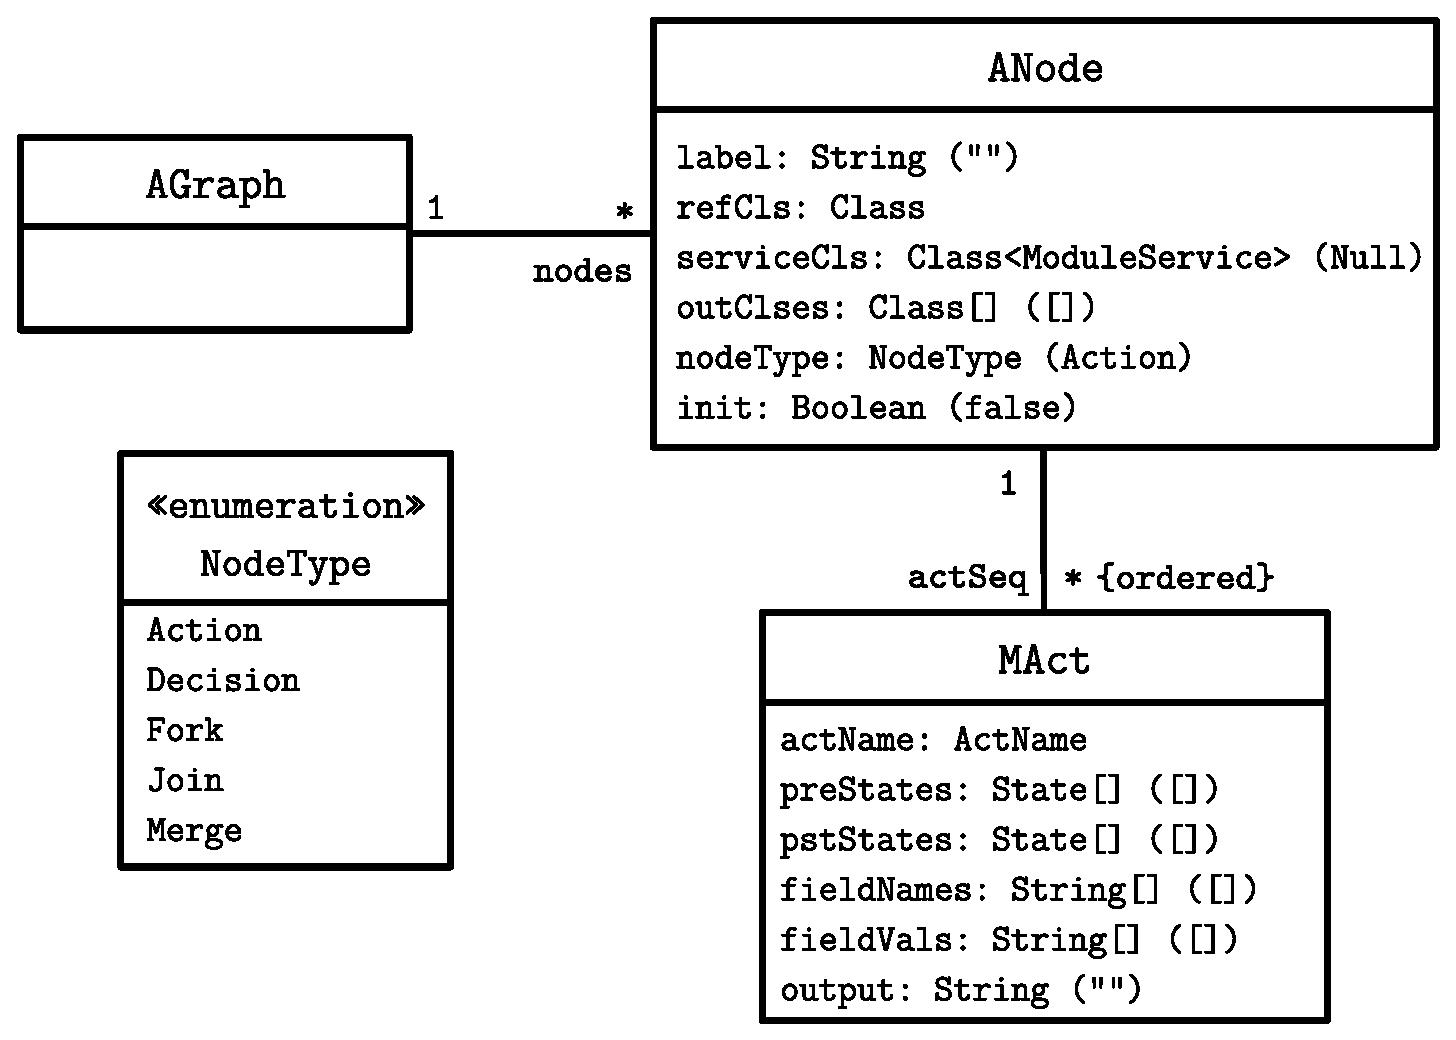
\includegraphics[scale=0.4]{agl-cmt}
	\end{center}
	\caption{CSM$_T$: a compact and annotation-friendly model.} %
	\label{fig:agl-csmt}
\end{figure*}

% TODO:   + validation function
Note that due to the restrictions on the data type of annotation property, fields of certain meta-concepts in the ASM are not translated directly to fields in the CSM$_T$. In these cases, however, we compensate for the information loss by adding OCL constraints to the corresponding meta-concepts of the CSM$_T$. These constraints are realized by validation functions that are performed on these meta-concepts, when they are translated into the annotation form.
%
\begin{description}
%\subsubsection*{\clazz{MAct}} %\label{sect:agl-csmt-mact}
\item[\clazz{MAct}.] \clazz{MAct} realizes \clazz{ModuleAct} using only the data types that are supported by annotation. Specifically, the data types of \attrib{MAct}{preStates} and \attribn{pstStates} (the latter is short for \attribn{postStates}) are arrays of \clazz{State}. The default values of these fields are an empty array (\code{[]}), which do not mean that they are not specified. An empty array in this case means that it takes the default state value of action as specified in Table~\ref{tab:core-atomic-actions} of Section~\ref{sect:arch-atomic-action}.
The following additional OCL constraints help ensure that the two fields contain unique values, which are required to match the \clazz{Set} data type of the two corresponding fields of \clazz{ModuleAct}.
% TODO: + MAct
% + OCL constraint on preStates, pstStates
\begin{lstrule}
-- MAct.preStates and pstStates (if specified) contain unique values
context Node inv:
  not(preStates.oclIsUndefined()) implies preStates->asSet() = preStates and 
  not(pstStates.oclIsUndefined()) implies pstStates->asSet() = pstStates
\end{lstrule}

As for the two fields \attrib{MAct}{fieldNames} and \attribn{fieldVals}, they also take an array type. This is equivalent to the \clazz{Seq} data type of the two corresponding fields of \clazz{ModuleAct}. Note that \attribn{fieldVals} is typed \clazz{String[]}, which requires that the value objects, if specified, are written explicitly as a string. Fortunately, this is not at all troublesome, because \attribn{fieldVals} is only required if the value objects are specified by the user. For many cases, however, the values come from another action or an external system. In these cases, \clazz{fieldVals} need not be specified and can take the default value of an empty array.

Last but not least, field \attrib{MAct}{output} is typed \clazz{String} and has the default value of an empty string (\strq{}). This field is added only for completeness. It always takes the default value, because the output value of a module action is never specified by the user. It is generated from within the system.
%
%\subsubsection*{\clazz{ANode}} \label{sect:agl-cmt-anode}
\item[\clazz{ANode}.] Class \clazz{ANode} both represents \clazz{Node} and \clazz{Edge} and merges the entire \clazz{ControlNode} type hierarchy. To achieve the former, we add to \clazz{ANode} a new field, named \membern{outClses}, that captures the \textit{ref} domain classes of the target nodes of the outgoing edges of a node. To achieve the latter, we add to \clazz{ANode} a field named \attribn{nodeType}, whose data type is the enumeration \clazz{NodeType}. This enumeration specifies all the pre-defined node types, including action and the control types.

%TODO: + ANode
% + add extra OCL constraints for the above
\begin{lstrule}
-- ANode.refCls and ANode.outClses (if specified) are domain classes
context Node inv:
  not(refCls.oclIsUndefined()) implies refCls.isDomainClass() and 
  not(outClses.oclIsUndefined()) implies outClses->forAll(isDomainClass())
\end{lstrule}

Note that we cannot explicitly define the data types of \attrib{ANode}{refCls} and \attribn{outClses} as parameterized types of \clazz{DomainClass}, because this class only exists in the ASM and not in the actual annotation-based model. We compensate for this information loss in the two data types by two OCL constraints on \clazz{ANode} for the two fields. Both constraints (listed immediately above) make use of a boolean function named \func{isDomainClass}. This function, which is defined as part of the ASM's library rules in~\ref{apex:agl-Class}, is invoked on a class to check if it is attached to a \clazz{DClass} element. 
%
%\subsubsection*{\clazz{AGraph}} \label{sect:agl-cmt-agraph}
\item[\clazz{AGraph}.] Class \clazz{AGraph} is simplified from \clazz{ActivityGraph} by having just one associative field for \clazz{ANode}. To further simplify this graph and ease its configuration, we replace the field \attrib{ActivityGraph}{n0} by a new boolean-typed field \attrib{ANode}{init}. We reconstruct \attrib{ActivityGraph}{n0} from all \clazz{ANode}s that have \attribn{init} = \code{true}.
\end{description}

%%%%%%%%%%%%%%%%%%%%%%%%%%%%%%%%%%%%%%%%%%%%%
\subsubsection{Mapping from ASM to CSM$_T$} \label{sect:agl-asm2csmt}
%%%%%%%%%%%%%%%%%%%%%%%%%%%%%%%%%%%%%%%%%%%%%
% TODO: + mapping asm-2-csmt
% + update based on the new ASM, CSMt
% + add bijective theorem
\begin{table}[ht]
	\centering
	\caption{Rules for mapping ASM $\rightarrow$ CSM$_T$} \label{tab:agl-asm2csmt}
	\footnotesize
	\setlength\tabcolsep{1pt}
	\begin{tabular}{|>{\centering\arraybackslash}m{0.5cm}|>{\centering\arraybackslash}m{8cm}|>{\centering\arraybackslash}m{7.5cm}|}\hline
		\rowcolor{lightgray}
		\multicolumn{1}{|c|}{\textbf{M\textit{Id}}} & 
		\multicolumn{1}{c|}{\textbf{ASM}} &
		\multicolumn{1}{c|}{$\mathbf{CSM_T}$} \\\hline
		%
		\ruledef{mruleno}{M}{Same} & \clazz{Decision}, \clazz{Join}, \clazz{ActName}, \clazz{State} & (same) \\\hline		
		%
		\ruledef{mruleno}{M}{MAct} & 
      \clazz{ModuleAct} & \clazz{MAct} \\\hline
    %
		\ruledef{mruleno}{M}{ANode} & \clazz{Node} & \clazz{ANode}{.}(\func{excl.})\attribn{nodeType},
%    \attribn{actSeq}, 
    \attribn{outClses}, \attribn{init} \\\hline
		%
		\ruledef{mruleno}{M}{DecisionNode} & \clazz{DecisionNode} & \objc{ANode}{\attribn{nodeType}=\code{Decision}} \\\hline
		%
		\ruledef{mruleno}{M}{ForkNode} & \clazz{ForkNode} & \objc{ANode}{\attribn{nodeType}=\code{Fork}} \\\hline
		%
		\ruledef{mruleno}{M}{JoinNode} & \clazz{JoinNode} & \objc{ANode}{\attribn{nodeType}=\code{Join}}\\\hline
		%
		\ruledef{mruleno}{M}{MergeNode} & \clazz{MergeNode} & \objc{ANode}{\attribn{nodeType}=\code{Merge}} \\\hline  
		%
%		\ruledef{mruleno}{M}{ANode.actSeq} & \attrib{ANode}{actSeq} & \clzassoc{\_}{Node}{ModuleAct} \\\hline
		%
		\ruledef{mruleno}{M}{ANode.outClses} & 
		$\funcdef{outClses}{\clazz{Node}}{\powerset{\clazz{Class}}}$ \linebreak
		($\forall n \in \clazz{Node}. n.\attribn{out} \neq \emptyset$). %\linebreak
		\func{outClses}($n$) = $ \{ c ~|~ c = e.n_{2}.\attribn{refCls}, $ \linebreak $e \in n.\attribn{out} \} $ & \attrib{ANode}{outClses} \\\hline
		%
		\ruledef{mruleno}{M}{ANode.init} & 
		$\funcdef{isInitNode}{\clazz{Node}}{\clazz{Boolean}}$ \linebreak
		($\forall n \in \clazz{Node}$). %\linebreak
		\func{isInitNode}($n$) = $ (n \in n.\attribn{graph}.\attribn{n0}) $ & \attrib{ANode}{init} \\\hline
		%
		\ruledef{mruleno}{M}{Edge} & \clazz{Edge} & 
		$ R_{edge}\subseteq \clazz{ANode} \times \clazz{ANode}, $ \linebreak 
		$ R_{edge} = \{ (a_1, a_2) ~|~ $ 
		$a_1, a_2 \in \clazz{ANode}, $ 
		$a_1.\attribn{outClses}.\attribn{length} > 0, $ 
		$a_2.\attribn{refCls} \in a_1.\attribn{outClses} \} $ \\\hline
		%
%		\ruledef{mruleno}{M}{GraphNodes} & \attrib{AGraph}{nodes} & \clzassoc{\Bigfilleddiamond}{ActivityGraph}{Node} \\\hline
%		%
%		\ruledef{mruleno}{M}{GraphEdges} & \ruleref{M}{Edge} \& \ruleref{M}{GraphNodes} & \clzassoc{\Bigfilleddiamond}{ActivityGraph}{Edge} \\\hline
		%
		\ruledef{mruleno}{M}{AGraph} & 
       \clazz{ActivityGraph} & \clazz{AGraph} \\\hline
		%
		\ruledef{mruleno}{M}{AGraphNodes} & 
       \attrib{ActivityGraph}{nodes} & \attrib{AGraph}{nodes} \\\hline
    \ruledef{mruleno}{M}{AGraphEdges} & \attrib{ActivityGraph}{edges} & 
      $\funcdef{edges}{\clazz{AGraph}}{\clazz{ANode} \times \clazz{ANode}}$ \linebreak
      ($\forall g \in \clazz{AGraph}$). %\linebreak
		\func{edges}($g$) =  $\{ (a_1, a_2) ~|~ a_1, a_2 \in g.\attribn{nodes}, a_2.\attribn{refCls} \in a_1.\attribn{outClses} \} $ \\\hline
    \ruledef{mruleno}{M}{AGraphN0} & \attrib{ActivityGraph}{n0} & 
      $\funcdef{initNodes}{\clazz{AGraph}}{\powerset{\clazz{ANode}}}$ \linebreak
      ($\forall g \in \clazz{AGraph}$). \func{initNodes}($g$) = $\{ a ~|~ a \in g.\attribn{nodes}, a.\attribn{init} = \code{true} \} $ \\\hline
	\end{tabular}
\end{table}

We explain in this section the precise transformation ASM $\rightarrow $ CSM$_T$ in terms of a set of mapping rules. Table~\ref{tab:agl-asm2csmt} lists definitions of these rules. 
%
Mapping rule \ruleref{M}{Same} is an identity map on \clazz{Decision}, \clazz{Join}, \clazz{ActName}, and \clazz{State}. These meta-concepts are transferred directly to CSM$_T$.
%
Given the additional OCL constraints that were defined previously on \clazz{MAct}, mapping rule \ruleref{M}{MAct} maps \clazz{ModuleAct} to \clazz{MAct}.

Mapping rules \ruleref{M}{ANode}--\ruleref{M}{ANode.init} define the mapping for \clazz{ANode}. Specifically, \ruleref{M}{ANode} maps \clazz{Node} to the field set of \clazz{ANode} that excludes (\func{excl.}) three fields (\attribn{nodeType}, \attribn{outClses}, and \attribn{init}). 
The other rules define mapping for these excluded fields. 
%
First, rules \ruleref{M}{DecisionNode}--\ruleref{M}{MergeNode} together map the four \clazz{ControlNode} subtypes to \attrib{ANode}{nodeType} (this field specifies four subsets of \clazz{ANode} objects). 
%
%Second, rule \ruleref{M}{ANode.actSeq} maps field \attrib{ANode}{actSeq} to the association between \clazz{Node} and \clazz{ModuleAct}.
%
Second, rule \ruleref{M}{ANode.outClses} maps to field \attrib{ANode}{outClses} a query function, named \func{outClses}, that returns a set of domain classes derived from the field \attrib{Node}{refCls} of the target nodes ($ n_2 $) of all the outgoing edges ($ n.\attribn{out} $) of a \clazz{Node} ($ n $). Here, \attrib{Node}{out}: \clazztemplate{Set}{\clazz{Edge}} is a derived field, whose value consists of all \clazz{Edge}s that have field \attribn{n1} equating the current node.
%
Third, rule \ruleref{M}{ANode.init} maps to field \attrib{ANode}{init} a boolean query function, named \func{isInitNode}, which returns \code{true} or \code{false} depending on whether a \clazz{Node} ($ n $) is the initial node of the \clazz{ActivityGraph} to which it belongs.

Rule \ruleref{M}{Edge} maps \clazz{Edge} to an ``edge'' relation on \clazz{ANode}, named $R_{edge}$, that returns a set of \clazz{ANode} pairs $ (a_1, a_2) $, each of which qualifies to form the (source, target) pair of an \clazz{Edge}: $a_2$'s \attribn{refCls} is one of the domain classes in $a_1$'s \attribn{outClses}.

Finally, rules \ruleref{M}{AGraph}--\ruleref{M}{AGraphN0} map \clazz{AGraph} to \clazz{ActivityGraph}. Rules \ruleref{M}{AGraph} and \ruleref{M}{AGraphNodes} map \clazz{ActivityGraph} to \clazz{AGraph} and \attrib{ActivityGraph}{nodes} to \attrib{AGraph}{nodes}, respectively. Rule \ruleref{M}{AGraphEdges} maps \attrib{ActivityGraph}{edges} to a query function, named \func{edges}, over \clazz{AGraph}, which returns a set of node tuples $(a_1, a_2)$ that form the edges. Rule \ruleref{M}{AGraphN0} maps \attrib{ActivityGraph}{n0} to another query function, named \func{initNodes} and is also over \clazz{AGraph}, which returns all the \clazz{ANode}s whose \attribn{init} = \code{true}.

From the language-engineering perspective, it is important to show that the mapping ASM $ \rightarrow $ CSM$_T$ is bijective. Bijective mapping~\cite{stevens_landscape_2008} means that CSM$_T$ has the same information capacity as ASM. Mathematically~\cite{weisstein_bijective_2018}, this also means that the mapping has an inverse or `backward' mapping. It is through this inverse mapping and an CSM that is derived from the CSM$_T$ (discussed in the next section) that we can generate the activity graph of an AGC, written in the textual syntax of a host OOPL.
%
\begin{theorem} \label{thm:mapping-cm2cmt}
Mapping ASM $\rightarrow$ CSM$_T$ is bijective, \ie for every ASM's instance, there exists exactly one CSM$_T$'s instance to which it is mapped. \qed 
\end{theorem}

\begin{proof}
Because each mapping rule in Table~\ref{tab:agl-asm2csmt} is applied independently, if we can prove that each of them is bijective, then the entire mapping ASM $\rightarrow$ CSM$_T$ is bijective. We provide below a brief proof of each mapping rule.

Rules \ruleref{M}{Same}--\ruleref{M}{MAct}: These are trivially bijective, because each preserves the information capacity of the relevant ASM's meta-concepts.

Rule \ruleref{M}{ANode}: This is bijective because it preserves the information capacity of \clazz{Node}. In particular, the additional OCL constraints that we introduced in \clazz{ANode} help preserve meanings of the data types of \attrib{Node}{refCls} and \attribn{serviceCls}.

Rule \ruleref{M}{DecisionNode}: This is bijective because of the following reasons. The node types captured in \clazz{NodeType} are unique. Thus, field \attrib{ANode}{nodeType} helps group \clazz{ANode}s into different disjoint subsets. In particular, for every \clazz{DecisionNode} $n$, there exists exactly one \clazz{ANode}, whose \attribn{nodeType} = \code{Decision} and other fields are set to the corresponding fields of $n$. 

Rules \ruleref{M}{ForkNode}--\ruleref{M}{MergeNode}: These are bijective by the arguments similar to the one presented above for \ruleref{M}{DecisionNode}.

Rule \ruleref{M}{ANode.outClses}: This rule shows how a new field \attrib{ANode}{outClses} is constructed from the function \func{outClses} over \clazz{Node}. To prove for this rule, we first assume there exists a derived field, \attrib{Node}{\_outClses}, whose extent is defined by the function \func{outClses}. The rule \ruleref{M}{ANode.outClses} then becomes the mapping rule \attrib{Node}{\_outClses} $ \rightarrow $ \attrib{ANode}{outClses}. This mapping rule is bijective by definition.

Rule \ruleref{M}{ANode.init}: This rule also involves constructing a new field (\attrib{ANode}{init}), whose extent is defined by a function (\func{isInitNode}) over \clazz{Node}. The proof thus proceeds similarly to the proof presented above for rule \ruleref{M}{ANode.outClses} (\ie using a derived field).

Rule \ruleref{M}{Edge}: We prove that for every \clazz{Edge} $ e = (n_1, n_2) $, there is (\textit{a}) one and (\textit{b}) only one pair of \clazz{ANode}s $ (a_1, a_2) \in R_{edge} $, such that $ n_1 \rightarrow a_1$ and $ n_2 \rightarrow a_2 $.

(\textit{a}): First, we select $a_1$ from $n_1$ by applying a suitable combination of the mapping rules \ruleref{M}{ANode}--\ruleref{M}{ANode.init}. Now, by construction, we have $ a_1.\attribn{outClses} = \func{outClses}(n_1) $. Because of \clazz{Edge} $ e $ we have: $n_2.\attribn{refCls} \in \func{outClses}(n_1)$. Thus, if we select $a_2$ from $n_2$ (by applying suitable mapping rules among \ruleref{M}{ANode}--\ruleref{M}{ANode.init}) then $a_2.\attribn{refCls} = n_2.\attribn{refCls} \in a_1.\attribn{outClses}$. In other words, $ (a_1, a_2) \in R_{edge} $.

(\textit{b}): The bijectiveness of the mapping rules \ruleref{M}{ANode}--\ruleref{M}{ANode.init} help guarantee this, because there is exactly one $ a_1 $ (\resp~$a_2$) \st $ n_1 \rightarrow a_1$ (\resp~$n_2 \rightarrow a_2$).

Rule \ruleref{M}{AGraph}: This is bijective by definition.

Rule \ruleref{M}{AGraphNodes}: This is bijective by definition.

Rule \ruleref{M}{AGraphEdges}: We prove this by assuming the existence of a derived field \attrib{AGraph}{\_edges}, whose extent is defined by the function \func{edges}. Then this mapping rule trivially becomes the bijective mapping between two fields: $ \attrib{ActivityGraph}{edges} \rightarrow \attrib{AGraph}{\_edges}$.

Rule \ruleref{M}{AGraphN0}: Similarly, this is proved by first assuming the existence of a derived field \attrib{AGraph}{\_initNodes}, whose extent is defined by the function \func{initNodes}. Then, the mapping between two fields ($ \attrib{ActivityGraph}{n0} \rightarrow \attrib{AGraph}{\_initNodes}$) is a bijective mapping.
\end{proof}

%%%%%%%%%%%%%%%%%%%%%%%%%%%%%%%%%%%%%%%%%%%%%%%
\subsubsection{The Annotation-Based CSM}
\label{sect:agl-csm}
%%%%%%%%%%%%%%%%%%%%%%%%%%%%%%%%%%%%%%%%%%%%%%%

Although CSM$_T$ is suitable for OOPL's representation, it is still not yet natively in that form. Our next step, therefore, is to transform it into a CSM that is ``embedded'' into OOPL. This CSM is constructed from the following three OOPL meta-concepts that were discussed in Section~\ref{sect:bg-dcsl}: class, annotation, and property.

\begin{figure*}[ht]
	\begin{center}
		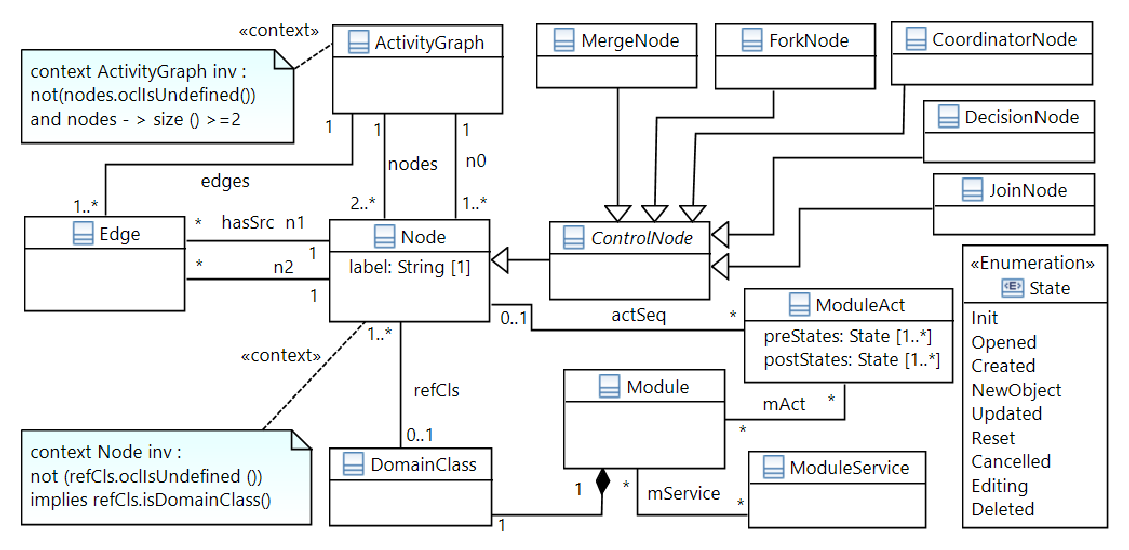
\includegraphics[scale=0.4]{agl-asm}
	\end{center}
	\caption{The concrete syntax model (CSM) of \agl.} %
	\label{fig:agl-csm}
\end{figure*}

Figure~\ref{fig:agl-csm} shows the metamodel in the formm of a UML class diagram for ASM. In this, the three meta-classes in CSM$_T$ are transformed into three annotations of the same name. The annotations are represented in the figure as 2-part grey-coloured boxes, the association lines as grey lines. Each domain field is transformed into an annotation property. The non-associative domain fields are transformed directly into properties and so, to ease reading, we use `\dots' to represent these properties. We only highlight in the figure two properties of the two associative fields \attrib{AGraph}{nodes} and \attrib{ANode}{actSeq}. 

A key difference between CSM and CSM$_T$ is the attachment of \clazz{AGraph} to \clazz{Class}. This is represented in Figure~\ref{fig:agl-csm} by a solid line connecting the two corresponding class boxes. An \clazz{AGraph} attachment defines an AGC because it describes the instantiation of an \clazz{AGraph} object together with the associated \clazz{ANode}s and \clazz{MAct} objects.

Adding the \clazz{AGraph} attachment to our definition of activity class (see Definition~\ref{def:unified-class-model}) helps form a bridge between \agl~and the unified model. More specifically, in the overall context of our method, we call any class that has an \clazz{AGraph} attachment an \textit{activity class}.
Further, to ease discussion we will use the term \textbf{configured unified model} to refer to a unified model whose the activity class is attached with an \clazz{AGraph}.

The following theorem ensures that \agl's CSM has the same information capacity as CSM$_T$ through the transformation.
%
\begin{theorem} \label{theo:csmt-csm}
The mapping CSM$_T$ $\rightarrow$ CSM is bijective. \qed
\end{theorem}
%
\begin{proof}
The proof of Theorem~\ref{theo:csmt-csm} is trivial as it follows directly from the fact that the CSM does not contain any new features and from the following two properties about the mapping. First,  each class in CSM$_T$ is bijectively mapped to one annotation in CSM. Second, each associative field in CSM$_T$ is bijectively mapped to an annotation property.
\end{proof}
%
\subsubsection*{Discussion} \label{sect:agl-discussion} %
In the current syntax, the AGC is sensibly attached to the activity class, because this class serves as the pivot for the activity graph definition.
%
An alternative annotation-based syntax would be to not define the \clazz{ANode}s as a property of \clazz{AGraph} (i.e., to remove property \attrib{AGraph}{nodes}), but to distribute them such that they are attached to the domain classes that they reference (via the property \attrib{ANode}{refCls}). 

However, this syntax has several limitations. First, we need extra properties in order to keep track of which \clazz{ANode}s belong to which \clazz{AGraph}. For example, we need two new properties \attrib{AGraph}{id} and \attrib{ANode}{graph}, the values of which in the same \clazz{AGraph} are equal. 
Second, it is more difficult to read, understand, and validate the AGC. This is because the AGC is not in one place but is scattered around in different parts of the domain model.
Third, we would unnecessarily complicate the component classes with \clazz{ANode} specifications, which in turn would hinder their use and understandability. These classes should only be concerned with the domain logics, not the mechanics of the activity graph that executes them.

%%%%%%%%%%%%%%%%%%%%%%%%%%%%%%%%%%%%%%%%%%%%%%%%%%%%%%%%%%%%%%%
\subsection{Annotation-Based Textual Concrete Syntax} 
\label{sect:agl-csSyntax}
%%%%%%%%%%%%%%%%%%%%%%%%%%%%%%%%%%%%%%%%%%%%%%%%%%%%%%%%%%%%%%%

Because CSM is embedded directly into OOPL, its structure helps define the core structure of a CSM model of the \agl's textual syntax. Adapting the concrete syntax meta-modeling approach~\cite{kleppe_software_2008} to \agl, we argue that its CSM will contain, in addition to the above core, meta-concepts that help describe the structure of the BNF grammar rules. The textual syntaxes of Java and C\# are both described using this grammar.
%
For exposition purpose in this paper, we will textually write an AGC using the structured note box notation of \dcsl~(explained in Section~\ref{sect:bg-dcsl}). The following example will help to illustrate.

\subsubsection*{Example: AGC and configured unified model}
\begin{figure}[ht]
	\begin{center}
		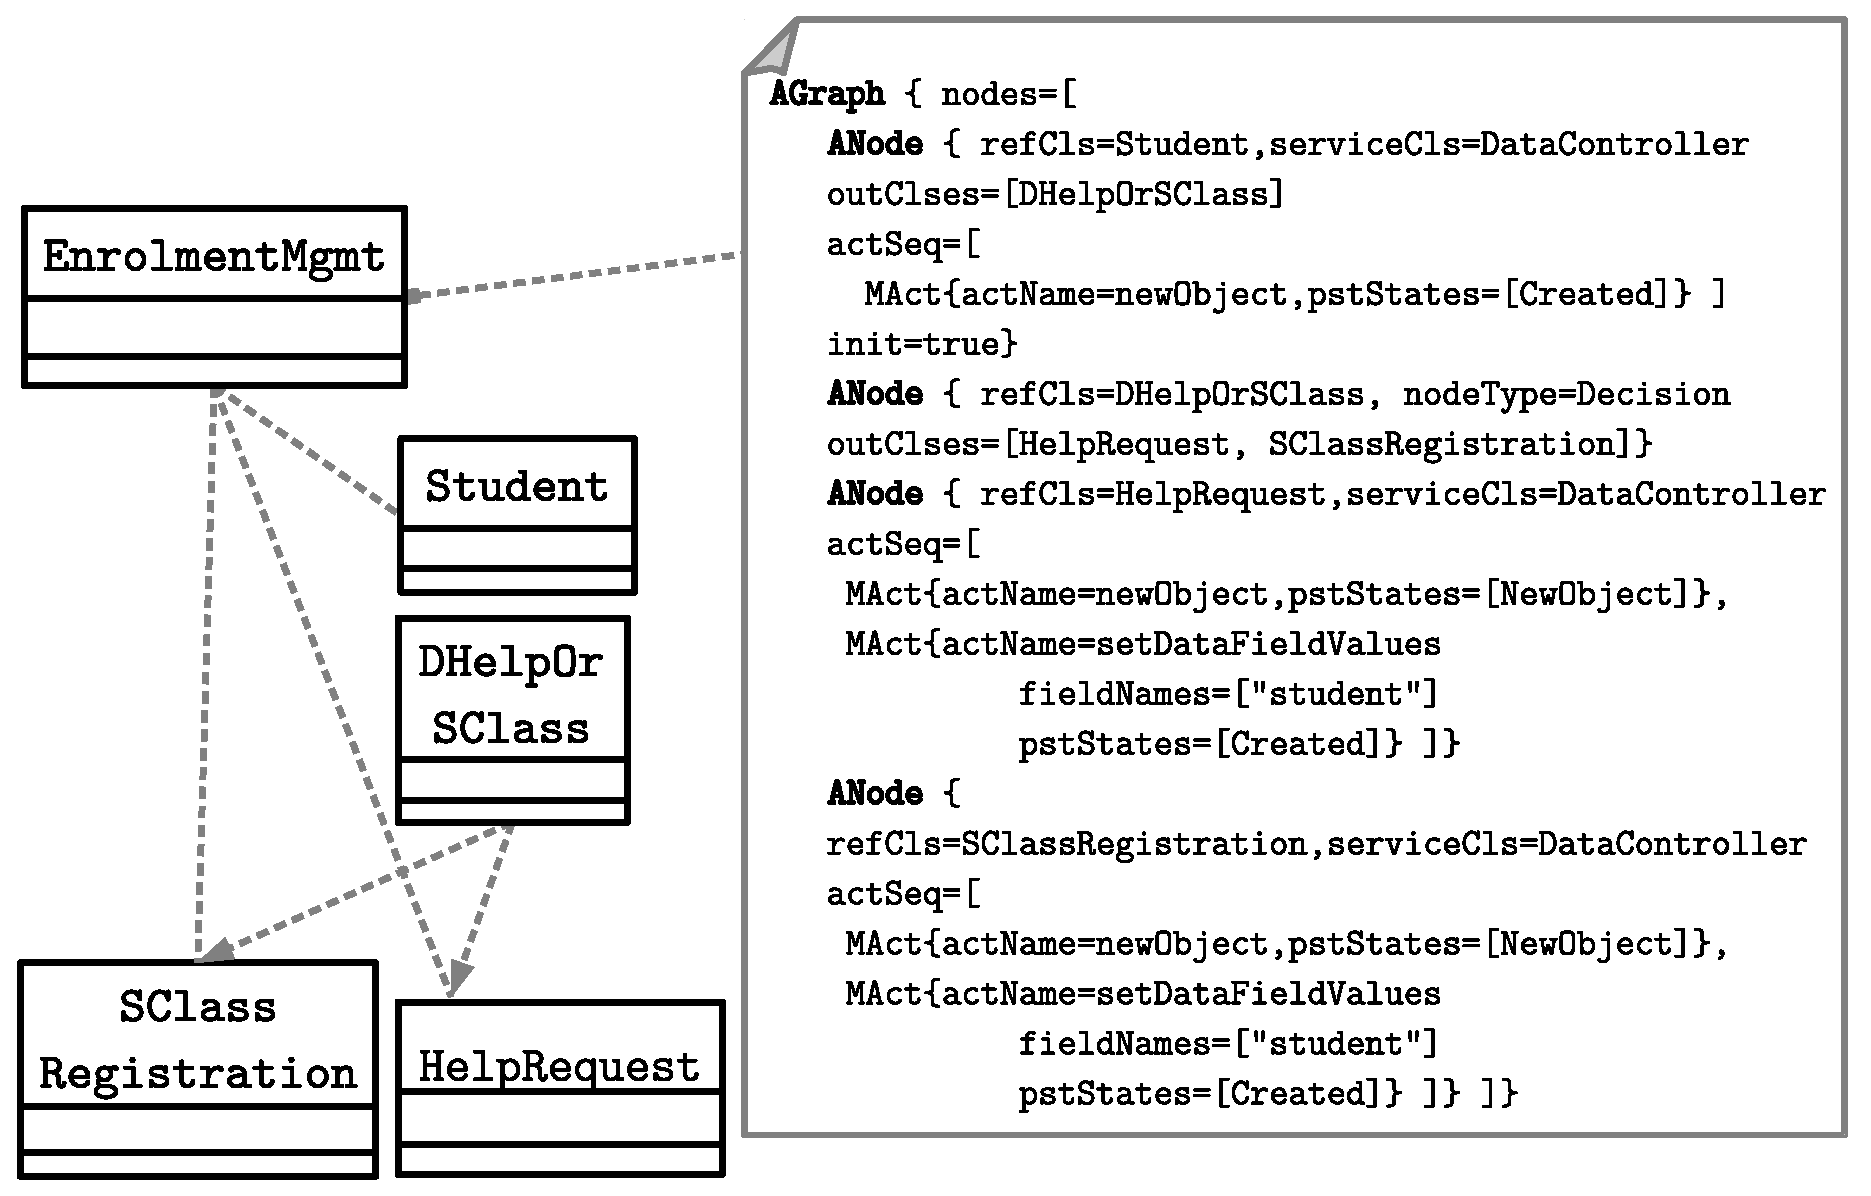
\includegraphics[scale=0.35]{agc-enrolmentmgmt}
	\end{center}
	\caption{Configured unified model of the enrolment management activity: (LHS) the unified model, (RHS) the AGC written in the annotation-based concrete syntax.} %
	\label{fig:agc-enrolmentmgmt}
\end{figure}

Figure~\ref{fig:agc-enrolmentmgmt} depicts the configured unified model of the enrolment management activity shown in  Figure~\ref{fig:activity-graph-example}. As shown in Figure~\ref{fig:agc-enrolmentmgmt}, the entire AGC is defined by an \clazz{AGraph} element, which is written within a note box attached to the activity class \clazz{EnrolmentMgmt} of the unified model.
%
As can be seen from the figure, the \clazz{AGraph} element is configured with its property \attribn{nodes} being set to an array of four \clazz{ANode}s. These \clazz{ANode}s configure the four \clazz{Node} objects listed earlier in Table~\ref{tab:activity-graph-example}, and additionally for each of them the component class(es) that will become the referenced domain classes of the target nodes of the outgoing edges (if any). These component class(es) are specified by property \attrib{ANode}{outClses}. For example, the first \clazz{ANode} configures the state of the node \objid{1}{Node}. Property \attribn{outClses} of this \clazz{ANode} is set to the array [\clazz{DHelpOrSClass}], which states that \objid{1}{Node} has an outgoing edge whose target node is the node whose \textit{ref} domain class is \clazz{DHelpOrSClass}. According to Table~\ref{tab:activity-graph-example} this is node \objid{2}{Node}, and the outgoing edge is \objid{1}{Edge}.

%%%%%%%%%%%%%%%%%%%%%%%%%%%%%%%%%%%%%%%%%%%%%%%%%%%%%%
\subsection{Semantics} \label{sect:agl-semantics}
%%%%%%%%%%%%%%%%%%%%%%%%%%%%%%%%%%%%%%%%%%%%%%%%%%%%%%

Because ASM, CSM$_T$, and the \agl's CSM have the same information capacity, we can discuss the \agl's semantics using any of these models. We choose ASM because it has a clearer conceptual structure. Based on this structure (see Figure~\ref{fig:agl-abstractSyntax}), we argue that the \agl's semantics is an extension of the core UML activity graph semantics to incorporate \clazz{ModuleAct} as a type of execution node. Indeed, Figure~\ref{fig:agl-abstractSyntax} shows that ASM consists in \clazz{ModuleAct} (positioned at the top of the figure) and the UML activity graph, scoped by the inclusion, exclusion and restriction clauses in Section~\ref{sect:agl-abstractSyntax}. The semantics of \clazz{ModuleAct} was discussed in Section~\ref{sect:actSemantics}, while the semantics of UML activity graph is defined informally in the UML specification~\cite{omg_unified_2015} itself and formally in~\cite{daw_extensible_2015}.

We conclude this section with an updated definition of the software generated in MOSA. This definition makes precise the general notion of module-based software that we introduced in Section~\ref{sect:bg-arch} and takes into account the combination of unified model and activity graph. It highlights the sub-set of modules that owns the activity classes and how these modules trigger the execution of the activity graphs of the associated activities.
%
\begin{definition} \label{def:software}
Given a unified model $D$ that contains a non-empty set of activity classes, each of which is attached to an AGC describing the activity graph logic of an activity in the UML activity model of the domain. A software generated in MOSA \wrt $D$ consists in a set of modules, each of which owns a domain class in $D$ and the behavior of the \code{newObject} action of every owner module of an activity class includes the logic described by the activity graph that is configured by the AGC attached to that class. \qed
\end{definition}



